
%% bare_conf.tex
%% V1.3
%% 2007/01/11
%% by Michael Shell
%% See:
%% http://www.michaelshell.org/
%% for current contact information.
%%
%% This is a skeleton file demonstrating the use of IEEEtran.cls
%% (requires IEEEtran.cls version 1.7 or later) with an IEEE conference paper.
%%
%% Support sites:
%% http://www.michaelshell.org/tex/ieeetran/
%% http://www.ctan.org/tex-archive/macros/latex/contrib/IEEEtran/
%% and
%% http://www.ieee.org/

%%*************************************************************************
%% Legal Notice:
%% This code is offered as-is without any warranty either expressed or
%% implied; without even the implied warranty of MERCHANTABILITY or
%% FITNESS FOR A PARTICULAR PURPOSE!
%% User assumes all risk.
%% In no event shall IEEE or any contributor to this code be liable for
%% any damages or losses, including, but not limited to, incidental,
%% consequential, or any other damages, resulting from the use or misuse
%% of any information contained here.
%%
%% All comments are the opinions of their respective authors and are not
%% necessarily endorsed by the IEEE.
%%
%% This work is distributed under the LaTeX Project Public License (LPPL)
%% ( http://www.latex-project.org/ ) version 1.3, and may be freely used,
%% distributed and modified. A copy of the LPPL, version 1.3, is included
%% in the base LaTeX documentation of all distributions of LaTeX released
%% 2003/12/01 or later.
%% Retain all contribution notices and credits.
%% ** Modified files should be clearly indicated as such, including  **
%% ** renaming them and changing author support contact information. **
%%
%% File list of work: IEEEtran.cls, IEEEtran_HOWTO.pdf, bare_adv.tex,
%%                    bare_conf.tex, bare_jrnl.tex, bare_jrnl_compsoc.tex
%%*************************************************************************

% *** Authors should verify (and, if needed, correct) their LaTeX system  ***
% *** with the testflow diagnostic prior to trusting their LaTeX platform ***
% *** with production work. IEEE's font choices can trigger bugs that do  ***
% *** not appear when using other class files.                            ***
% The testflow support page is at:
% http://www.michaelshell.org/tex/testflow/



% Note that the a4paper option is mainly intended so that authors in
% countries using A4 can easily print to A4 and see how their papers will
% look in print - the typesetting of the document will not typically be
% affected with changes in paper size (but the bottom and side margins will).
% Use the testflow package mentioned above to verify correct handling of
% both paper sizes by the user's LaTeX system.
%
% Also note that the "draftcls" or "draftclsnofoot", not "draft", option
% should be used if it is desired that the figures are to be displayed in
% draft mode.
%
\documentclass[conference]{IEEEtran}
% Add the compsoc option for Computer Society conferences.
%
% If IEEEtran.cls has not been installed into the LaTeX system files,
% manually specify the path to it like:
% \documentclass[conference]{../sty/IEEEtran}





% Some very useful LaTeX packages include:
% (uncomment the ones you want to load)


% *** MISC UTILITY PACKAGES ***
%
%\usepackage{ifpdf}
% Heiko Oberdiek's ifpdf.sty is very useful if you need conditional
% compilation based on whether the output is pdf or dvi.
% usage:
% \ifpdf
%   % pdf code
% \else
%   % dvi code
% \fi
% The latest version of ifpdf.sty can be obtained from:
% http://www.ctan.org/tex-archive/macros/latex/contrib/oberdiek/
% Also, note that IEEEtran.cls V1.7 and later provides a builtin
% \ifCLASSINFOpdf conditional that works the same way.
% When switching from latex to pdflatex and vice-versa, the compiler may
% have to be run twice to clear warning/error messages.






% *** CITATION PACKAGES ***
%
%\usepackage{cite}
% cite.sty was written by Donald Arseneau
% V1.6 and later of IEEEtran pre-defines the format of the cite.sty package
% \cite{} output to follow that of IEEE. Loading the cite package will
% result in citation numbers being automatically sorted and properly
% "compressed/ranged". e.g., [1], [9], [2], [7], [5], [6] without using
% cite.sty will become [1], [2], [5]--[7], [9] using cite.sty. cite.sty's
% \cite will automatically add leading space, if needed. Use cite.sty's
% noadjust option (cite.sty V3.8 and later) if you want to turn this off.
% cite.sty is already installed on most LaTeX systems. Be sure and use
% version 4.0 (2003-05-27) and later if using hyperref.sty. cite.sty does
% not currently provide for hyperlinked citations.
% The latest version can be obtained at:
% http://www.ctan.org/tex-archive/macros/latex/contrib/cite/
% The documentation is contained in the cite.sty file itself.






% *** GRAPHICS RELATED PACKAGES ***
%
\ifCLASSINFOpdf
  % \usepackage[pdftex]{graphicx}
  % declare the path(s) where your graphic files are
  % \graphicspath{{../pdf/}{../jpeg/}}
  % and their extensions so you won't have to specify these with
  % every instance of \includegraphics
  % \DeclareGraphicsExtensions{.pdf,.jpeg,.png}
\else
  % or other class option (dvipsone, dvipdf, if not using dvips). graphicx
  % will default to the driver specified in the system graphics.cfg if no
  % driver is specified.
  % \usepackage[dvips]{graphicx}
  % declare the path(s) where your graphic files are
  % \graphicspath{{../eps/}}
  % and their extensions so you won't have to specify these with
  % every instance of \includegraphics
  % \DeclareGraphicsExtensions{.eps}
\fi
% graphicx was written by David Carlisle and Sebastian Rahtz. It is
% required if you want graphics, photos, etc. graphicx.sty is already
% installed on most LaTeX systems. The latest version and documentation can
% be obtained at:
% http://www.ctan.org/tex-archive/macros/latex/required/graphics/
% Another good source of documentation is "Using Imported Graphics in
% LaTeX2e" by Keith Reckdahl which can be found as epslatex.ps or
% epslatex.pdf at: http://www.ctan.org/tex-archive/info/
%
% latex, and pdflatex in dvi mode, support graphics in encapsulated
% postscript (.eps) format. pdflatex in pdf mode supports graphics
% in .pdf, .jpeg, .png and .mps (metapost) formats. Users should ensure
% that all non-photo figures use a vector format (.eps, .pdf, .mps) and
% not a bitmapped formats (.jpeg, .png). IEEE frowns on bitmapped formats
% which can result in "jaggedy"/blurry rendering of lines and letters as
% well as large increases in file sizes.
%
% You can find documentation about the pdfTeX application at:
% http://www.tug.org/applications/pdftex





% *** MATH PACKAGES ***
%
%\usepackage[cmex10]{amsmath}
% A popular package from the American Mathematical Society that provides
% many useful and powerful commands for dealing with mathematics. If using
% it, be sure to load this package with the cmex10 option to ensure that
% only type 1 fonts will utilized at all point sizes. Without this option,
% it is possible that some math symbols, particularly those within
% footnotes, will be rendered in bitmap form which will result in a
% document that can not be IEEE Xplore compliant!
%
% Also, note that the amsmath package sets \interdisplaylinepenalty to 10000
% thus preventing page breaks from occurring within multiline equations. Use:
%\interdisplaylinepenalty=2500
% after loading amsmath to restore such page breaks as IEEEtran.cls normally
% does. amsmath.sty is already installed on most LaTeX systems. The latest
% version and documentation can be obtained at:
% http://www.ctan.org/tex-archive/macros/latex/required/amslatex/math/





% *** SPECIALIZED LIST PACKAGES ***
%
%\usepackage{algorithmic}
% algorithmic.sty was written by Peter Williams and Rogerio Brito.
% This package provides an algorithmic environment fo describing algorithms.
% You can use the algorithmic environment in-text or within a figure
% environment to provide for a floating algorithm. Do NOT use the algorithm
% floating environment provided by algorithm.sty (by the same authors) or
% algorithm2e.sty (by Christophe Fiorio) as IEEE does not use dedicated
% algorithm float types and packages that provide these will not provide
% correct IEEE style captions. The latest version and documentation of
% algorithmic.sty can be obtained at:
% http://www.ctan.org/tex-archive/macros/latex/contrib/algorithms/
% There is also a support site at:
% http://algorithms.berlios.de/index.html
% Also of interest may be the (relatively newer and more customizable)
% algorithmicx.sty package by Szasz Janos:
% http://www.ctan.org/tex-archive/macros/latex/contrib/algorithmicx/




% *** ALIGNMENT PACKAGES ***
%
%\usepackage{array}
% Frank Mittelbach's and David Carlisle's array.sty patches and improves
% the standard LaTeX2e array and tabular environments to provide better
% appearance and additional user controls. As the default LaTeX2e table
% generation code is lacking to the point of almost being broken with
% respect to the quality of the end results, all users are strongly
% advised to use an enhanced (at the very least that provided by array.sty)
% set of table tools. array.sty is already installed on most systems. The
% latest version and documentation can be obtained at:
% http://www.ctan.org/tex-archive/macros/latex/required/tools/


%\usepackage{mdwmath}
%\usepackage{mdwtab}
% Also highly recommended is Mark Wooding's extremely powerful MDW tools,
% especially mdwmath.sty and mdwtab.sty which are used to format equations
% and tables, respectively. The MDWtools set is already installed on most
% LaTeX systems. The lastest version and documentation is available at:
% http://www.ctan.org/tex-archive/macros/latex/contrib/mdwtools/


% IEEEtran contains the IEEEeqnarray family of commands that can be used to
% generate multiline equations as well as matrices, tables, etc., of high
% quality.


%\usepackage{eqparbox}
% Also of notable interest is Scott Pakin's eqparbox package for creating
% (automatically sized) equal width boxes - aka "natural width parboxes".
% Available at:
% http://www.ctan.org/tex-archive/macros/latex/contrib/eqparbox/





% *** SUBFIGURE PACKAGES ***
%\usepackage[tight,footnotesize]{subfigure}
% subfigure.sty was written by Steven Douglas Cochran. This package makes it
% easy to put subfigures in your figures. e.g., "Figure 1a and 1b". For IEEE
% work, it is a good idea to load it with the tight package option to reduce
% the amount of white space around the subfigures. subfigure.sty is already
% installed on most LaTeX systems. The latest version and documentation can
% be obtained at:
% http://www.ctan.org/tex-archive/obsolete/macros/latex/contrib/subfigure/
% subfigure.sty has been superceeded by subfig.sty.



%\usepackage[caption=false]{caption}
%\usepackage[font=footnotesize]{subfig}
% subfig.sty, also written by Steven Douglas Cochran, is the modern
% replacement for subfigure.sty. However, subfig.sty requires and
% automatically loads Axel Sommerfeldt's caption.sty which will override
% IEEEtran.cls handling of captions and this will result in nonIEEE style
% figure/table captions. To prevent this problem, be sure and preload
% caption.sty with its "caption=false" package option. This is will preserve
% IEEEtran.cls handing of captions. Version 1.3 (2005/06/28) and later
% (recommended due to many improvements over 1.2) of subfig.sty supports
% the caption=false option directly:
%\usepackage[caption=false,font=footnotesize]{subfig}
%
% The latest version and documentation can be obtained at:
% http://www.ctan.org/tex-archive/macros/latex/contrib/subfig/
% The latest version and documentation of caption.sty can be obtained at:
% http://www.ctan.org/tex-archive/macros/latex/contrib/caption/




% *** FLOAT PACKAGES ***
%
%\usepackage{fixltx2e}
% fixltx2e, the successor to the earlier fix2col.sty, was written by
% Frank Mittelbach and David Carlisle. This package corrects a few problems
% in the LaTeX2e kernel, the most notable of which is that in current
% LaTeX2e releases, the ordering of single and double column floats is not
% guaranteed to be preserved. Thus, an unpatched LaTeX2e can allow a
% single column figure to be placed prior to an earlier double column
% figure. The latest version and documentation can be found at:
% http://www.ctan.org/tex-archive/macros/latex/base/



%\usepackage{stfloats}
% stfloats.sty was written by Sigitas Tolusis. This package gives LaTeX2e
% the ability to do double column floats at the bottom of the page as well
% as the top. (e.g., "\begin{figure*}[!b]" is not normally possible in
% LaTeX2e). It also provides a command:
%\fnbelowfloat
% to enable the placement of footnotes below bottom floats (the standard
% LaTeX2e kernel puts them above bottom floats). This is an invasive package
% which rewrites many portions of the LaTeX2e float routines. It may not work
% with other packages that modify the LaTeX2e float routines. The latest
% version and documentation can be obtained at:
% http://www.ctan.org/tex-archive/macros/latex/contrib/sttools/
% Documentation is contained in the stfloats.sty comments as well as in the
% presfull.pdf file. Do not use the stfloats baselinefloat ability as IEEE
% does not allow \baselineskip to stretch. Authors submitting work to the
% IEEE should note that IEEE rarely uses double column equations and
% that authors should try to avoid such use. Do not be tempted to use the
% cuted.sty or midfloat.sty packages (also by Sigitas Tolusis) as IEEE does
% not format its papers in such ways.





% *** PDF, URL AND HYPERLINK PACKAGES ***
%
%\usepackage{url}
% url.sty was written by Donald Arseneau. It provides better support for
% handling and breaking URLs. url.sty is already installed on most LaTeX
% systems. The latest version can be obtained at:
% http://www.ctan.org/tex-archive/macros/latex/contrib/misc/
% Read the url.sty source comments for usage information. Basically,
% \url{my_url_here}.





% *** Do not adjust lengths that control margins, column widths, etc. ***
% *** Do not use packages that alter fonts (such as pslatex).         ***
% There should be no need to do such things with IEEEtran.cls V1.6 and later.
% (Unless specifically asked to do so by the journal or conference you plan
% to submit to, of course. )


% correct bad hyphenation here
%\hyphenation{op-tical net-works semi-conduc-tor}


\begin{document}
%
% paper title
% can use linebreaks \\ within to get better formatting as desired
\title{StreamDiv Project Report}


% author names and affiliations
% use a multiple column layout for up to three different
% affiliations
%\author{\IEEEauthorblockN{Michael Shell}
%\IEEEauthorblockA{School of Electrical and\\Computer Engineering\\
%Georgia Institute of Technology\\
%Atlanta, Georgia 30332--0250\\
%Email: http://www.michaelshell.org/contact.html}
%\and
%\IEEEauthorblockN{Homer Simpson}
%\IEEEauthorblockA{Twentieth Century Fox\\
%Springfield, USA\\
%Email: homer@thesimpsons.com}
%\and
%\IEEEauthorblockN{James Kirk\\ and Montgomery Scott}
%\IEEEauthorblockA{Starfleet Academy\\
%San Francisco, California 96678-2391\\
%Telephone: (800) 555--1212\\
%Fax: (888) 555--1212}}

% conference papers do not typically use \thanks and this command
% is locked out in conference mode. If really needed, such as for
% the acknowledgment of grants, issue a \IEEEoverridecommandlockouts
% after \documentclass

% for over three affiliations, or if they all won't fit within the width
% of the page, use this alternative format:
%
\author{\IEEEauthorblockN{Steve,
Nick,
Nathan Ong,
Zaeem,
Panos Chrysanthis and
Alexandros Labrinidis}
\IEEEauthorblockA{Department of Computer Science\\
University of Pittsburgh,
Pittsburgh, Pennsylvania 15260\\ Email: }
}




% use for special paper notices
%\IEEEspecialpapernotice{(Invited Paper)}




% make the title area
\maketitle


\begin{abstract}
%\boldmath
Data mountains continue to grow in size, increasing the difficulty in retrieving useful analysis from them.  In addition, generated data is frequently plagued by sameness; the data that is retrieved tends to follow the same pattern, helpful in simple prediction tasks or outlier detection, but not necessarily helpful in characterizing the data from a stream.  Users tend to know in a general sense what they are searching for in their datasets and streams, but may not know the full space of relevant results.  Diversity helps alleviate this problem, but faces its own challenges when combined with relevancy and recency in streaming contexts.\\
\indent In our work, we explore different designs for a diversity operator in a stream processing environment.  In addition, we factor in the impact of recency and user-defined relevancy by ranking incoming data.  Users will specify a size for a representative top-$k$ set for the data seen from the stream.  This top-$k$ set is maintained by the system and updated based on recency, relevancy, and diversity from continuous streaming data.  We consider two types of tuple-replacement schemes, Incremental and Batch, for maintaining the top-$k$ set, and find CONCLUSION.
\end{abstract}
% IEEEtran.cls defaults to using nonbold math in the Abstract.
% This preserves the distinction between vectors and scalars. However,
% if the conference you are submitting to favors bold math in the abstract,
% then you can use LaTeX's standard command \boldmath at the very start
% of the abstract to achieve this. Many IEEE journals/conferences frown on
% math in the abstract anyway.

% no keywords




% For peer review papers, you can put extra information on the cover
% page as needed:
% \ifCLASSOPTIONpeerreview
% \begin{center} \bfseries EDICS Category: 3-BBND \end{center}
% \fi
%
% For peerreview papers, this IEEEtran command inserts a page break and
% creates the second title. It will be ignored for other modes.
\IEEEpeerreviewmaketitle


\section{Introduction}

Data creation and collection only continues to increase, leaving a large burden on analysts to come up with a way to quickly and efficiently comb through the data to locate trends and correlations.  There tends to be a focus on data-specific approaches with frameworks that work well for certain kinds of data (but not well on others CITATION NEEDED).  There also is a need in data analysis to provide relevant but diverse data points as a digest of the full data set.  Several offline versions have been created \cite{Ge:2015:PD:2795218.2795224} CITATIONS NEEDED, but lack the speed to work in a streaming environment.  We present StreamDiv, a streaming framework built on top of a previously developed diversity system for offline database systems, PrefDiv\cite{Ge:2015:PD:2795218.2795224}, to provide queriers of a data streaming systems a top-$k$ set that is most relevant and diverse, adding recency as a possible influence on the digested set.

The system
model of our work is a stand-alone stream processing system, with a single
stream of data as input. Processing is modeled as a pipeline of operators,
which process incoming tuples and forward results to the next operator.
The output is not a single result (as in the case of traditional databases),
but periodical results that reflect the most sensible outcome (according
to the algorithm) based on time-windows.\\

\indent As far as different dimensions of the problem are concerned, ranking is
considered as a set of user-defined properties that are either attached to
incoming tuples (annotate), or are used for filtering out tuples. Turning
to the diversity operator, we abstract it as a stateful operator, with time-
based sliding windows. The operator's frequency of result production
can be one of the following: (i) a temporary snapshot of the most diverse
tuples in the current time-window produced every time a tuple is received,
(ii) a set of the most diverse tuples among all the tuples that have been
received in a user-defined epoch. In the latter case, we consider how
many tuples are replaced and which ones every time a new tuple arrives.
For the former case, we consider a static approach (a pre-defined fraction
p of the tuples are replaced after every epoch), and a dynamic one (the
fraction p of the tuples replaced is proportional to the $\delta$ in diversity gained
compared to the replacement fraction of the previous epoch). As regards
to replacement policy, we have the alternatives of random replacement,
and least recently tuple received replacement.
\section{Preliminaries}
Both diversity and relevance have been explored to quite some depth within the broader context of \textit{representative data exploration} techniques. The diversity of a set of tuples is usually defined using a distance measure between pairs of tuples. In the case of numerical attributes, this could be the Euclidean distance between the data points, whereas in other cases, this could be a function specific to the type of data we are dealing with. Formally, let $d(t_i,t_j)$ denote the distance between two tuples $t_i$ and $t_j$. One possible measure of diversity of a set $S$ is the sum of pairwise distance of all the points in $S$ and is defined as
\begin{equation}div(S) = \sum_{i=1}^{|S|}\sum_{j>i}^{|S|}d(t_i,t_j)\end{equation}
The objective of diversification algorithms is the pick a subset $S*$ with a fixed size $k$ from a larger set $D$ such that the diversity of set $S*$ is maximum. In other words
\begin{equation}S^{*}=\underset{S\subseteq D, |S|=k}{argmax} div(S)\end{equation}
Such an optimization problem has been shown to be NP hard. Several heuristics, however, have been proposed in the research literature that aim to achieve diversity close to the optimal.
While diversity in general is not query specific, the relevance of a set $S$ is usually based on the similarity of the tuples in $S$ to the user query posed to the database. Again, for numerical attributes, this similarity could be the proximity of a tuple to a desired, possibly non-existent, tuple or point in the sample space as per the user query. The overall relevance of the set $S$ is usually defined as the sum of the individual relevance scores of the points within the set. 
Techniques to extract representative data that is most diverse and also contains relevant results usually employ the MMR, or the Maximum Marginal Relevance, scheme, in which the objective function is the weighted sum of the diversity and relevance score of the subset. As both diversity and relevance are orthogonal, and sometimes conflicting, objectives, the weights in these schemes are usually pre specified based on problem requirements and properties of the dataset.

Most of the literature focuses on the problem of diversification and relevancy in the framework of traditional databases, where the data is stored on a disk and all of the data is available to the representative data extraction algorithm as it looks through the entire haystack to pick out a small \textit{representative} subset. The luxury of looking at the entire dataset is not afforded in a streaming system where the system only sees incoming windows of tuples and has to process them on the fly. The incoming data is not stored in its entirety because, at high input rates, the amount of data would quickly exceed the storage capacity. Even if the system has enough storage space to store all the data that it receives, the timing requirements in the streaming system are quite strict. The algorithm would be required to produce the top k attributes at fixed intervals and looking at the entire dataset may take enough time that the system fails to meet its deadline. In this work we look at the problem of diversification and relevance maximization in the context of streaming databases and develop schemes that would work in an online setting, producing high quality results at fixed intervals or as soon as new tuples arrive in the system.

Another aspect that becomes more prominent in streaming systems is the recency of the tuples produced. There may be applications that would prefer to see more recent results at the expense of diversity and/or relevance. One reason for this could be to observe trends in user tweets, for example in the case of twitter data. Our schemes also include the recency of tuples as an objective. We also explore the tradeoff between all these three objectives and their impact on the quality of results produced. 
\section{Problem Definition}

/**********This is the original Github version of Problem Definition *********/
\indent As far as different dimensions of the problem are concerned, ranking is
considered as a set of user-defined properties that are either attached to
incoming tuples (annotate), or are used for filtering out tuples. Turning
to the diversity operator, we abstract it as a stateful operator, with time-
based sliding windows. The operator's frequency of result production
can be one of the following: (i) a temporary snapshot of the most diverse
tuples in the current time-window produced every time a tuple is received,
(ii) a set of the most diverse tuples among all the tuples that have been
received in a user-defined epoch. In the latter case, we consider how
many tuples are replaced and which ones every time a new tuple arrives.
For the former case, we consider a static approach (a pre-defined fraction
p of the tuples are replaced after every epoch), and a dynamic one (the
fraction p of the tuples replaced is proportional to the $\delta$ in diversity gained
compared to the replacement fraction of the previous epoch). As regards
to replacement policy, we have the alternatives of random replacement,
and least recently tuple received replacement.


/**********This is the dropbox version of Problem Definition *********/
Consider a streaming system where a batch of tuples arrives at fixed intervals. The number of tuples within the batch could be different at different times. Consider one such batch, denoted by $N$, that arrives at time $t$ containing $n$  tuples. The tuples within the batch are represented as $N=\{t_1,t_2,...,t_n\}$. The system already maintains a set of $k$ tuples, where $k$ is fixed, that are representative of all the previous incoming batches. This set, denoted $T$, is represented as $T=\{\mathbf{t_1},\mathbf{t_2},...,\mathbf{t_k}\}$. The task is then to decide which of the tuples from $N$ should be  added to $T$ and, consequently, which tuples in $T$ should be discarded to keep the size of $T$ equal to $k$ while also keeping the \textit{quality} of $T$ as high as possible. The \textit{quality} of $T$, in our context, is the combined objective of three factors:
\begin{enumerate}
\item the diversity of tuples within $T$, 
\item the relevance of the tuples to the original query, and 
\item the amount of time elapsed since those tuples were generated, with more recent tuples given higher priority
\end{enumerate}
\section{Preliminary Experiments}

In this section we present some initial results we 
gathered from our preliminary experiments. 
We used Apache Storm v$0.9.4$ and Java 
OpenJDK v1.7. The topology we utilized in our experiments 
consisted of a Relevancy operator, followed by a 
Diversity Operator. 
As far as our dataset is concerned, 
we gathered tweets using Twitter's Streaming API, 
and accumulated $75000$ tweets. 
Even though the Streaming API provides a 
plethora of attributes for each Tweet, we 
kept only the creation date and the text. 
The reason for that is because those are 
the only attributes important for our experiments 
(creation date for recency and text for relevance). 
During the gathering process, we ignored tweets 
that had non-ASCII characters, since those do 
not contain usable information and posed 
problems in storage.

In order to get a first impression on StreamDiv's 
effectiveness, we decided to compare it with the 
offline version. 
We compare StreamDiv with the offline implementation 
of combined relevance-and-diversity, which is named 
PrefDiv. The latter performs the same 
algorithm, but it reads data from a database 
and has a global view of the tweets. 
Our experiments were designed in a way to measure 
StreamDiv's performance on (i) diversity, (ii) relevance, 
and (iii) intensity.

For diversity, we calculated for each pair of tweets 
the Cosine Similarity distance. There is no particular 
reason that we opted for the previous metric, and the 
usage of alternative distances is orthogonal to our 
experiments. In terms of relevance, we used a simple 
approach, which annotated each tweet with a score, 
based on a given set of keywords. 
The score is just the number of 
keywords found in the text of the tweet. 

\begin{figure}[t]
\centering
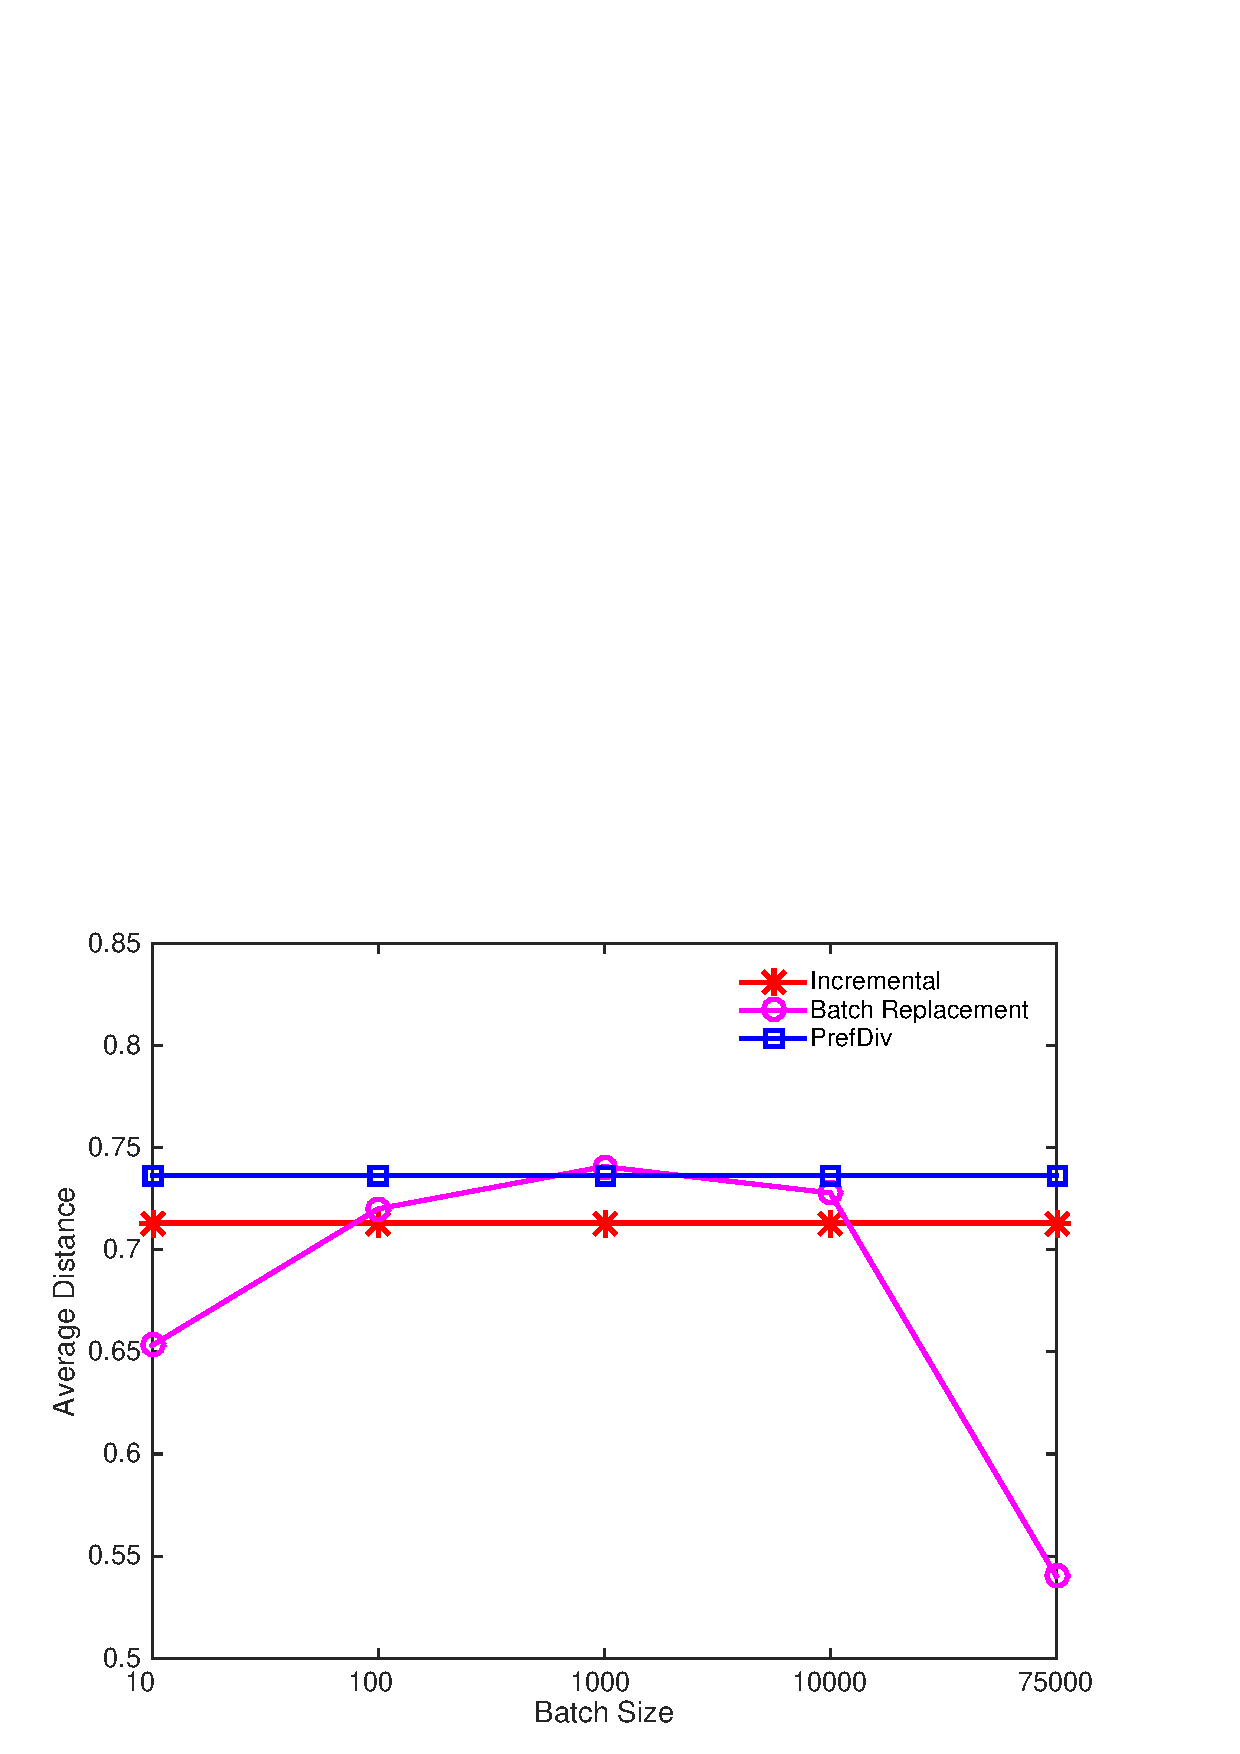
\includegraphics[width=0.4\textwidth,height=0.4\textheight,keepaspectratio]{AverageDistance.pdf}
\caption{Average Distance on different batch windows.}
\label{fig:avg-distance}
\end{figure}

Figure~\ref{fig:avg-distance} depicts the average distance 
achieved by using different batch sizes on StreamDiv. 
The incremental version of StreamDiv is not affected by 
the batch size, because it will always replace the 
same percentage of elements on every tuple. 
Therefore, the distance remains constant. 
The previous happens also in 
relevance and intensity. 
Turning to the batch version of StreamDiv, it is interesting 
how greater batch sizes, produce worse results in terms of diversity. 
The degradation of diversity is expected since the replacement 
policy of our prototype is naive at this point. 
In detail, the same percentage of tuples 
is discarded at every epoch. Hence, even if we achieve 
higher diversity at some point, a large number of tuples 
will be discarded, and the average distance will drop.

\begin{figure}[t]
\centering
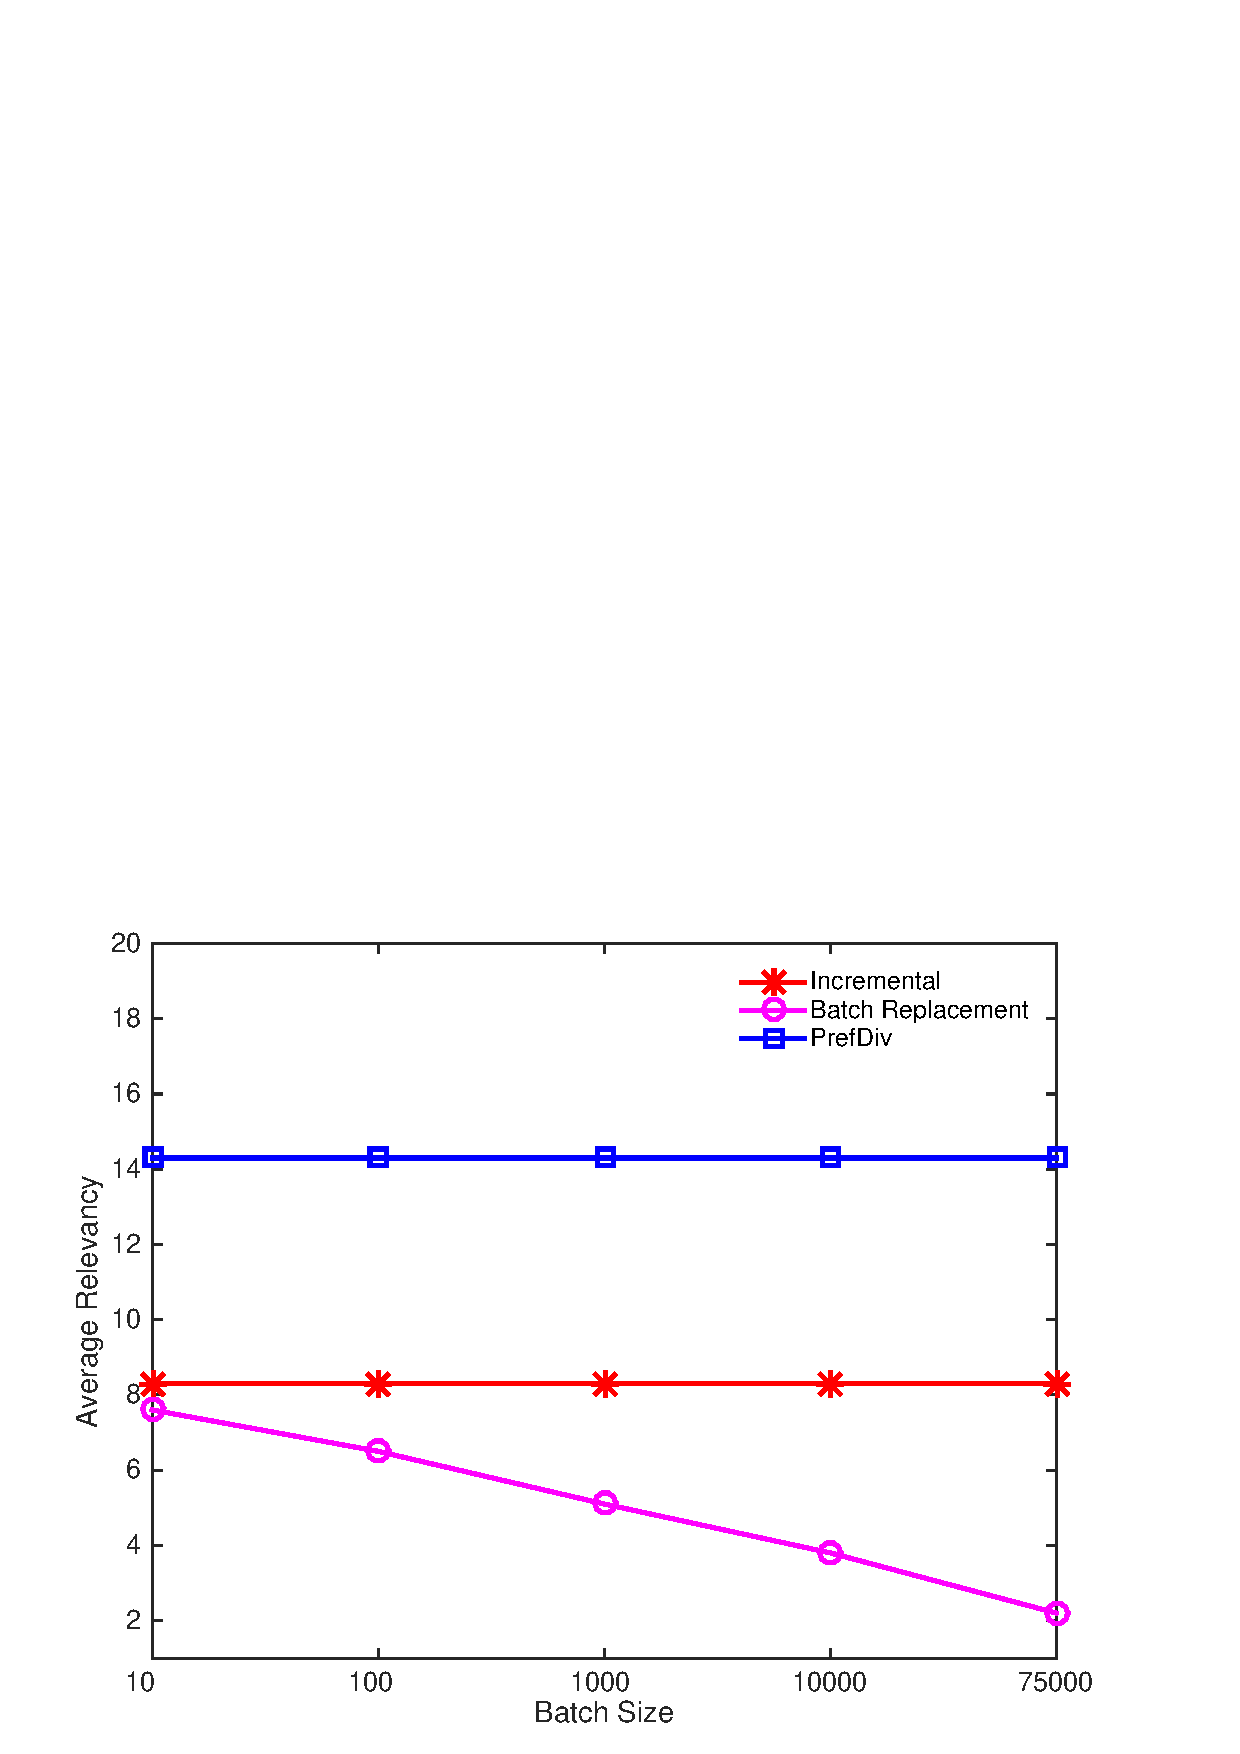
\includegraphics[width=0.4\textwidth,height=0.4\textheight,keepaspectratio]{AverageRelevancy.pdf}
\caption{Average Relevancy on different batch windows.}
\label{fig:avg-relevancy}
\end{figure}

Turning to relevance, we monitored similar results with 
average distance (depicted in Fig.~\ref{fig:avg-relevancy}). 
The number of tuples that will be replaced 
increases with the batch size. Therefore, the batch approach 
will more likely throw away important tuples. 
The same story appears in normalized intensity (see Figure~\ref{fig:norm-intensity}).
We expect that with the dynamic reconfiguration of the 
percentage, we will achieve better results.

\begin{figure}[t]
\centering
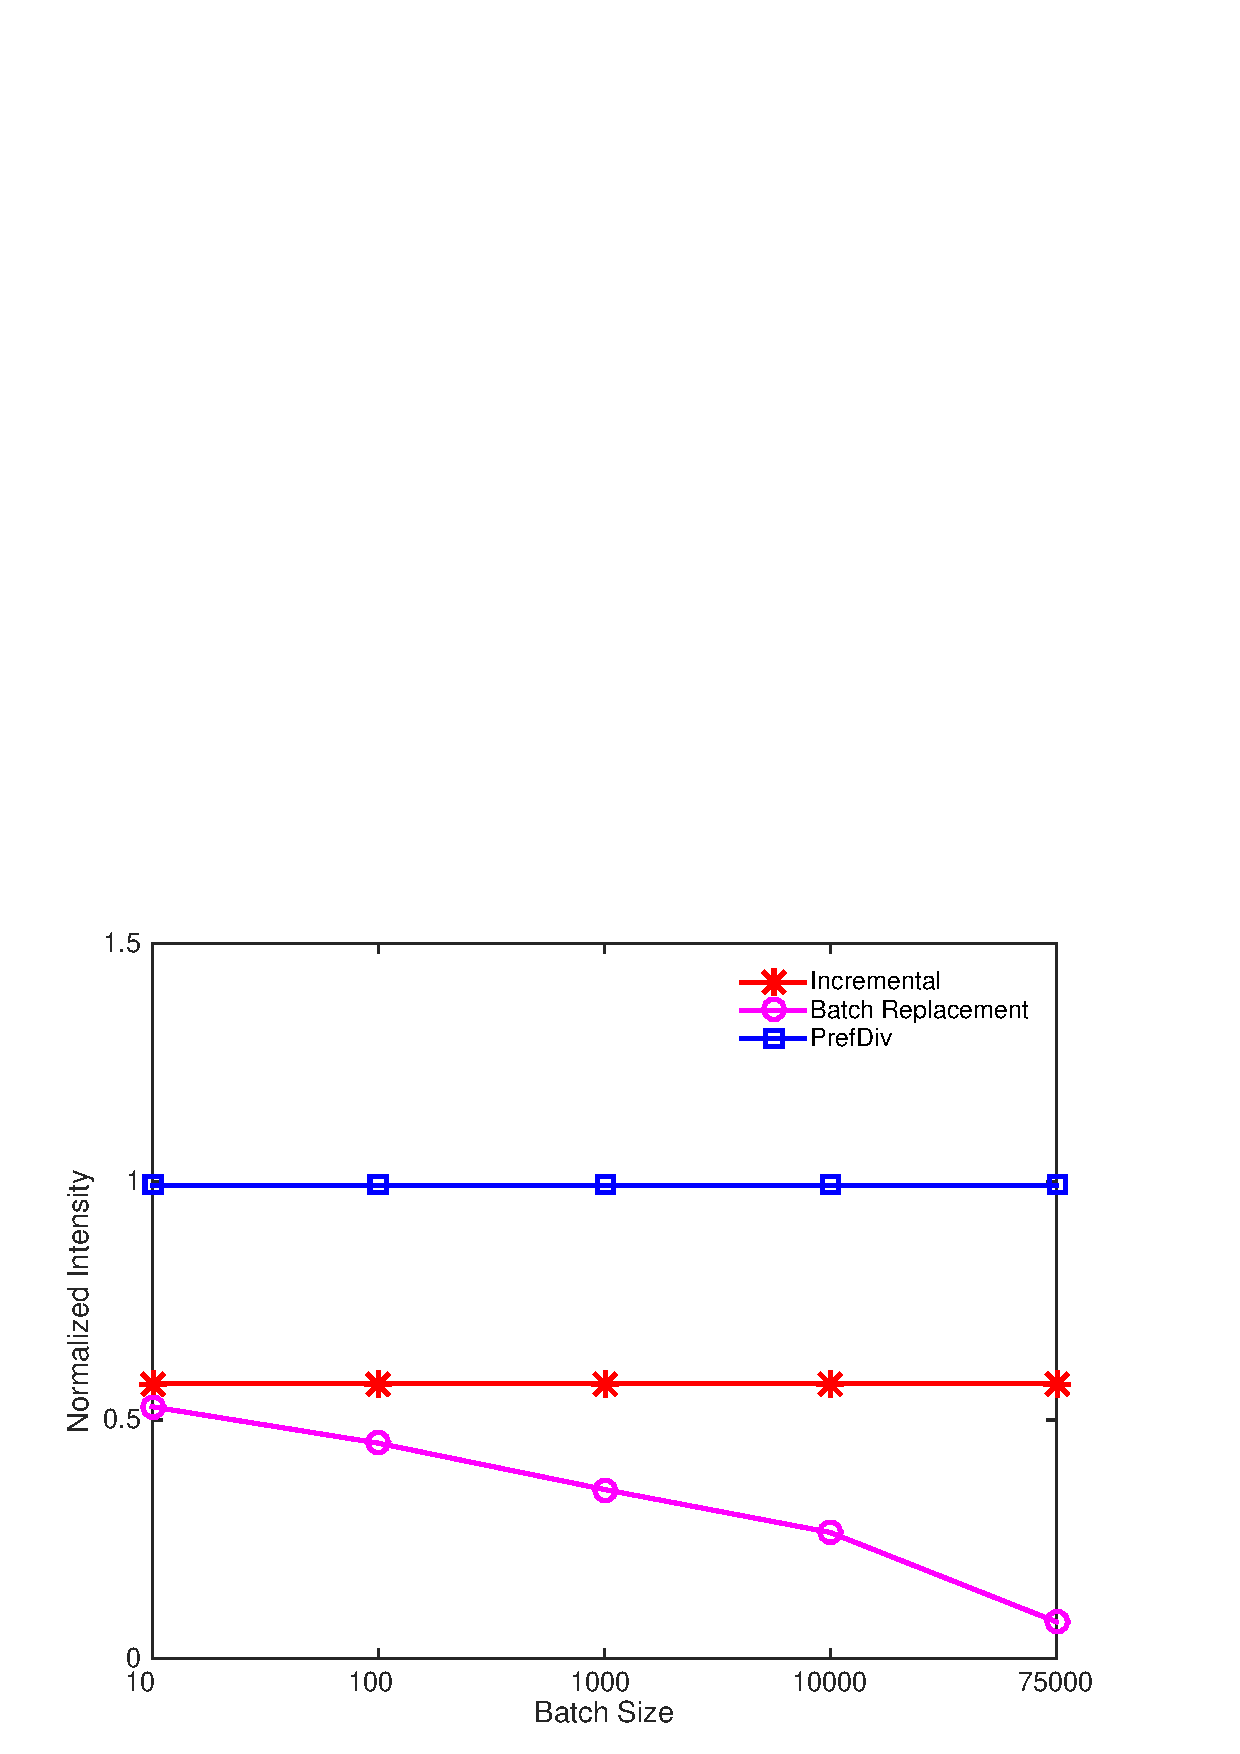
\includegraphics[width=0.4\textwidth,height=0.4\textheight,keepaspectratio]{NormalizedIntensity.pdf}
\caption{Normalized Intensity on different batch windows.}
\label{fig:norm-intensity}
\end{figure}

\section{Road Map}

List of things that need to be done:
\begin{enumerate}
\item	Implement dynamic reconfiguration of p for batch approach
\item	Implement smarter batch replacement policy
\item	Re-run experiments for a larger dataset.
\end{enumerate} 
\section{Results}
\section{Future work} 

In order for the paper to be published, below are list of things that we believe need to be improved:

\subsection{Implement dynamic reconfiguration of p for batch approach}

In order to make the windows replacement scheme work, we defined p as the coefficient of replacement, such that $0 \leq p \leq 1$. For every newly incoming window $w_1$, $k*p$ tuples from the top-k set will be replaced with the tuple in $w_1$. One naive way to implement the $p$ is to choose a fixed number, so that for every new window we only replace a fixed portion of tuples. However the drawback for this type of approach is obvious, as it is almost impossible to find the optimal $p$ that suits every input steam and window. In order to overcome this drawback, we purpose to implement a dynamic coefficient of replacement, such that:

\begin{equation}
  f(p) = (\dfrac{Score_{new}}{Score_{old}}) * p
\end{equation}

\begin{equation}
  p =
  \begin{cases}
    f(p) & \text{if $0 \leq p \leq 1$}\\
    p & \text{if otherwise}\\
   \end{cases}
\end{equation}

Where $Score_{new}$ is the total score for all tuples in the new windows and $Score_{old}$ is the total score for all tuples in the old windows.

By adopt the dynamic coefficient of replacement, StreamDiv will be able to reflect the underlying trends of changes of intensity value for all successor windows.

\subsection{Implement smarter batch replacement policy}

As the performs of StreamDiv will be heavily depends on the policy of how we conduct batch replacement, we need to carefully study the best way to perform the batch replacement. Currently, we only adopted a very naive approach for the batch replacement policy, in which for every newly incoming window we will run the incremental replacement algorithm $k * p$ times. Such replacement policy does not guarantee the optimal performance.

In order to improvement the performance of the batch replacement policy. We purpose to implement following scheme. For each batch $b_i$, once a newly incoming tuple from $b_i$ are being insert into the top-k set, we will mark it as non-removable, so that it will not be replaced by any tuple that are also from $b_i$ even if it is a neighbors of other successor tuples in $b_i$. This way we can ensure a desired amount of tuples will be replaced for every batch, and instead of stop the replacement for current batch when $k * p$ times incremental algorithm are performed, the replacement will keeping running until $k*p$ tuples are being replaced. This way, the number of tuples being replaced in this windows will be more closely bind with the coefficient of replacement p. We believe by adopting both smarter batch replacement policy and dynamic reconfiguration we will be able to significantly improve the perform of StreamDiv.

\subsection{Re-run experiments for a larger dataset.}

One thing we have to admit is that our current experiment are very preliminary, since we have only used 75000 tweets as our current data set for the experiment, and our current data set are gathered using only the stop words (e.g. the, a, is) as keywords, hence the data set is lacking focuses. In order to improve our experiment we purpose to use more meaningful keywords along with more tweets data. So that the experiment can have greater convincingness. 

Moreover, currently we only measure the statistics (e.g. average distance, normalized intensity and average relevancy) of the final result of each model, which means we only calculate all of the statistics once for the final top-k list of each model after the entire excitation is finished. However, for the future work, we would like to measure the average performance over each batch for both incremental and batch replacement models for different batch sizes. With this more detailed set of experiments, the performance different between different models can be more clear. 


\section{Future Work}
sadlkfjafk



% An example of a floating figure using the graphicx package.
% Note that \label must occur AFTER (or within) \caption.
% For figures, \caption should occur after the \includegraphics.
% Note that IEEEtran v1.7 and later has special internal code that
% is designed to preserve the operation of \label within \caption
% even when the captionsoff option is in effect. However, because
% of issues like this, it may be the safest practice to put all your
% \label just after \caption rather than within \caption{}.
%
% Reminder: the "draftcls" or "draftclsnofoot", not "draft", class
% option should be used if it is desired that the figures are to be
% displayed while in draft mode.
%
%\begin{figure}[!t]
%\centering
%\includegraphics[width=2.5in]{myfigure}
% where an .eps filename suffix will be assumed under latex,
% and a .pdf suffix will be assumed for pdflatex; or what has been declared
% via \DeclareGraphicsExtensions.
%\caption{Simulation Results}
%\label{fig_sim}
%\end{figure}

% Note that IEEE typically puts floats only at the top, even when this
% results in a large percentage of a column being occupied by floats.


% An example of a double column floating figure using two subfigures.
% (The subfig.sty package must be loaded for this to work.)
% The subfigure \label commands are set within each subfloat command, the
% \label for the overall figure must come after \caption.
% \hfil must be used as a separator to get equal spacing.
% The subfigure.sty package works much the same way, except \subfigure is
% used instead of \subfloat.
%
%\begin{figure*}[!t]
%\centerline{\subfloat[Case I]\includegraphics[width=2.5in]{subfigcase1}%
%\label{fig_first_case}}
%\hfil
%\subfloat[Case II]{\includegraphics[width=2.5in]{subfigcase2}%
%\label{fig_second_case}}}
%\caption{Simulation results}
%\label{fig_sim}
%\end{figure*}
%
% Note that often IEEE papers with subfigures do not employ subfigure
% captions (using the optional argument to \subfloat), but instead will
% reference/describe all of them (a), (b), etc., within the main caption.


% An example of a floating table. Note that, for IEEE style tables, the
% \caption command should come BEFORE the table. Table text will default to
% \footnotesize as IEEE normally uses this smaller font for tables.
% The \label must come after \caption as always.
%
%\begin{table}[!t]
%% increase table row spacing, adjust to taste
%\renewcommand{\arraystretch}{1.3}
% if using array.sty, it might be a good idea to tweak the value of
% \extrarowheight as needed to properly center the text within the cells
%\caption{An Example of a Table}
%\label{table_example}
%\centering
%% Some packages, such as MDW tools, offer better commands for making tables
%% than the plain LaTeX2e tabular which is used here.
%\begin{tabular}{|c||c|}
%\hline
%One & Two\\
%\hline
%Three & Four\\
%\hline
%\end{tabular}
%\end{table}


% Note that IEEE does not put floats in the very first column - or typically
% anywhere on the first page for that matter. Also, in-text middle ("here")
% positioning is not used. Most IEEE journals/conferences use top floats
% exclusively. Note that, LaTeX2e, unlike IEEE journals/conferences, places
% footnotes above bottom floats. This can be corrected via the \fnbelowfloat
% command of the stfloats package.








% conference papers do not normally have an appendix


% use section* for acknowledgement
\section*{Acknowledgment}


The authors would like to thank...





% trigger a \newpage just before the given reference
% number - used to balance the columns on the last page
% adjust value as needed - may need to be readjusted if
% the document is modified later
%\IEEEtriggeratref{8}
% The "triggered" command can be changed if desired:
%\IEEEtriggercmd{\enlargethispage{-5in}}

% references section

% can use a bibliography generated by BibTeX as a .bbl file
% BibTeX documentation can be easily obtained at:
% http://www.ctan.org/tex-archive/biblio/bibtex/contrib/doc/
% The IEEEtran BibTeX style support page is at:
% http://www.michaelshell.org/tex/ieeetran/bibtex/
\begin{small}
\bibliographystyle{IEEEtran}
% argument is your BibTeX string definitions and bibliography database(s)
\bibliography{IEEEabrv,references}
\end{small}
%
% <OR> manually copy in the resultant .bbl file
% set second argument of \begin to the number of references
% (used to reserve space for the reference number labels box)
%\begin{thebibliography}{1}
%
%\bibitem{IEEEhowto:kopka}
%H.~Kopka and P.~W. Daly, \emph{A Guide to \LaTeX}, 3rd~ed.\hskip 1em plus
%  0.5em minus 0.4em\relax Harlow, England: Addison-Wesley, 1999.
%
%\end{thebibliography}




% that's all folks
\end{document}


